%part1.tex
\part{背景知识}

\section{简介}\label{sec:introduction}
当 Knuth 编写 \TeX\ 的时候,还没有 \prgname{PostScript}/\prgname{eps}、\prgname{jpeg}、\prgname{gif} 以及其它图像格式。
\marginpar{历史渊源}
因此 \prgname{dvi} 文件对于图像导入并没有直接的支持。
不过,\TeX{} 允许\file{dvi} 文件中包含 \cmd{spectial} 命令,
通过它可以向调用 \file{dvi} 文件的程序传递命令。
因此,凡是调用 \file{dvi} 的程序支持的图像格式,
\TeX\ 和 \LaTeX\ 都能够导入。

过去的许多年来,\file{dvi} 通常都被转为 \file{PostScript}格式,
进而标准的插图格式是 Encapsulated PostScript(\file{eps})图像,
因为它是PostScript语言的一个子集。
在 \LaTeX{} 中插入\file{eps}图像最初通过低层命令 \cmd{spectial} 来完成。
为了使插图更加方便并且更具有可移植性,
专门为 \LaTeX 2.09 设计了两个高层的宏包 \pkg{epsf} 和 \pkg{psfig}。
\textsf{epsf}~提供了 \cmd{epsfbox} 命令来插入图片,
此外另有三个命令来控制图片的缩放。
在 \pkg{psfig} 中,\cmd{psfig} 命令除了用来插入图片,还有缩放和旋转功能。
不过,尽管 \pkg{psfig} 的句法更受欢迎,它的代码却没有 \pkg{epsf} 健壮。
于是作为这两个宏包的结合的产物,
\pkg{epsfig} 宏包使用 \pkg{psfig} 的句法和大部分 \pkg{epsf} 的健壮代码。
不过,\pkg{epsfig} 仍然使用了一些不健壮的 \pkg{psfig} 代码。

随着 1994 年 \LaTeXe{} 的发布,\LaTeX 3 小组认识到在 \LaTeX{} 中插图的一些普遍问题。
\marginpar{\LaTeX{} 图形宏集}
通过努力,他们开发出了“\LaTeX\ 图形宏集”,
\footnote{已经有 \LaTeX{} 图形宏集的 plain \TeX{} 版本,
	相关文件请见 \href{ftp://ctan.tug.org/tex-archive/macros/plain/graphics/}{CTAN/macros/generic/graphics/}}
其中的命令全部重写。
比起其它的插入命令,他们的命令更高效、更健壮、更具有可移植性。

\LaTeX{} 图形宏集包括“标准”的 \pkg{graphics} 宏包和“扩展”的 \pkg{graphicx} 宏包。
这两个宏包都有一个 \cmd{includegraphis} 命令,不过版本不同。
类似 \pkg{psfig} 的句法,
\pkg{graphicx} 版的 \cmd{includegraphis} 采用“命名参数(named arguments)”。
这使用起来比较简单方便,却违反了 \LaTeX{} 关于可选参数放置位置的语法指南方针。
作为折中方案,就有了两种版本的 \cmd{includegraphis}。
其中,\pkg{graphics} 的版本遵从 \LaTeX{} 的语法规则,
而\pkg{graphicx} 的版本则采用更为简便的命名参数。
\pkg{graphicx} 版本的 \cmd{includegraphis} 支持图形的缩放和旋转,
而 \pkg{graphics} 版本的 \cmd{includegraphis} 则必须被置于 \cmd{scalebox} 或 \cmd{rotatebox} 才能达到同样的效果。

本文档使用 \pkg{graphicx} 宏包,因为它的句法比 \pkg{graphics} 宏包更加简便易用。
其实这两个宏包具有相同的功能,本文档中的例子同样可以用 \pkg{graphics} 宏包完成,
只不过相应的命令有些笨拙和缺少一点效率。
关于这两个宏包详细的说明可参见 \LaTeX{} 图形宏集的文档~\cite{grfguide}。

出于向后兼容性,\LaTeX\ 图形宏包套件中也提供了一个 \pkg{epsfig} 宏包,
用以替代之前 \LaTeXe\ 的 \pkg{epsfig}。
新的\pkg{epsfig} 定义了 \cmd{epsfbox}、\cmd{psfig} 和 \cmd{epsfig} 等命令。
不过它们只是调用 \cmd{includegraphics} 命令的简单封装。
由于这些封装效率没有直接使用 \cmd{includegraphics} 命令高,
因此,该 \pkg{epsfig} 宏包应当只用于旧文档。
在编写新文档时要用 \cmd{includegraphics}。

除了改进 \file{eps} 图片的部分,\LaTeX{}~图形宏集还处理非 \file{eps} 图像格式的插图问题,
例如\file{jpeg} 和 \file{gif}等。
\marginpar{非 \file{eps} 图形}
由于 \file{dvi} 到 \file{ps} 的转换程序一般不直接支持大部分的非\file{eps} 格式,
向 \file{PostScript} 文档中插入这些图像之前相关图像必须首先转成 \file{eps} 格式。
尽管这种图像格式的预处理通常是最佳办法,
不过,\LaTeX\ 图形宏集还提供了另一种选择:\file{dvi} 转 \file{ps} 时自动地实时转换图像格式。
第 \ref{ssec:convertor} 节(\pageref{ssec:convertor} 页)介绍了一下图像转换程序,
第 \ref{sec:noneps} 节(\pageref{sec:noneps} 页) 讲述了如何在 \file{dvi} 转 \file{ps} 时使用非 \file{eps} 格式的图像。

过去,\file{PostScript} 通常是 \LaTeX{} 文档的最终格式,
\marginpar{\pdfTeX}
整个编译过程有两个步骤:
(1) 使用 \LaTeX{} 生成 \file{dvi} 文件,
(2) 使用一个 \file{dvi} 到 \file{ps} 的转换程序(例如\prgname{dvips}) 来生成 \file{PostScript} 文件。
之后,随着 Adobe 的 \file{pdf} 格式开始流行,编译过程又加了第三步:
(3) 使用 \prgname{Ghostscript}
\footnote{自由软件,见第 \ref{ssec:ghostscript} 节(\pageref{ssec:ghostscript} 页)。}、
\prgname{Adobe Acrobat}
\footnote{商业软件,见 \url{www.adobe.com}}
或者 \prgname{PStill}
\footnote{共享软件,见 \url{www.pstill.com}}
等工具将 \file{PostScript} 文件转成 \file{pdf} 文件。

然而,这种三步骤过程 \LaTeX-\prgname{dvips}-\prgname{ghostscript} 不仅很繁琐,
而且很难实现一些 \file{pdf} 特性,比如超链接。
为了改进这一点,Hàn Thế Thành 写了一个工具叫做 \TeX2PDF,
这一工具修改了 \TeX\ 引擎,可以直接从 \TeX{} 生成 \file{pdf}。
\TeX2PDF 最终重命名为 \pdfTeX,
并且在许多志愿者的帮助下(托高德纳的福)进行扩展,
进而实现了 \TeX{} 的全部排版功能。
\pdfTeX 从名称上看来输出的是 \file{pdf},
不过它也能输出 \file{dvi} 格式,并且与原先 \TeX{} 引擎的输出结果相同。

如同 \prgname{latex} 命令使用 \TeX{} 处理 \LaTeX{} 文档来生成 \file{dvi} 文件,
\prgname{pdflatex} 命令使用 \pdfTeX{} 处理 \LaTeX{} 文档,并直接生成 \file{pdf} 文件。
 
\pdfTeX{} 的一个重要特性就是原生支持许多图像格式:
\marginpar{\pdfTeX{} 和图像}
\file{jpeg}、\file{png}、\file{pdf}、\file{MetaPost}。
尽管老版本的 \pdfTeX{} 还支持 \file{tiff} 文件,目前的 \pdfTeX{} 版本不支持 \file{tiff}。

另外要注意的是,\pdfTeX{} 不能直接导入 \file{eps} 文件
\footnote{\pdfTeX{} 可以导入由 \prgname{PurifyEPS} 处理的 \file{eps} 文件,
	见第 \ref{ssec:purifyeps} 节(\pageref{ssec:purifyeps} 页)。},
用户需要用 \prgname{epstopdf} 等程序将 \file{eps} 文件转成 \file{pdf} 格式,
不过这样就不能直接使用 PSfrag 宏包(见第 \ref{sec:psfrag} 节,\pageref{sec:psfrag} 页)。

\section{\LaTeX{} 术语}\label{sec:terminology}

任何 \LaTeX{} 对象(字符,图形等)都把\emphi{盒子}作为单位(\cite[page 103]{Leslie})。
每个盒子在它的左侧均有一个\emphi{参考点}(\emphi{Reference point})。
盒子的\emphi{基线}(\emphi{baseline},见图~\ref{fig:samplebox})是一条通过参考点的
一条水平线。
当 \LaTeX{} 从左到右排列文本时,
每一字符的参考点排成一条水平直线,称为\emphi{当前基线}(\emphi{current baseline}),
并使它与字符的基线对齐。
\LaTeX{} 也用同样的方法来处理图形和其它对象,每个对象的参考点都被放置于当前基线上。

\begin{figure}
	\centering
	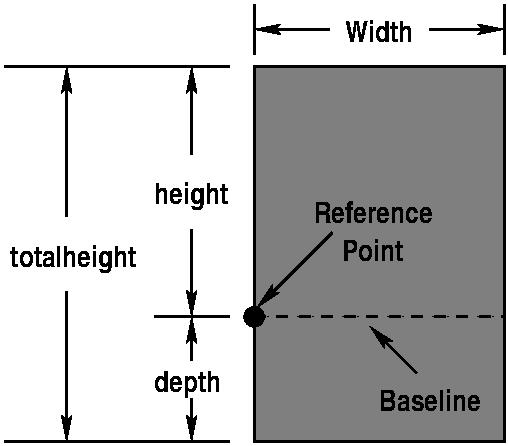
\includegraphics[width=.4\linewidth]{latex-box}
	\caption{\LaTeX{}~盒子示例}
	\label{fig:samplebox}
\end{figure}

每一个盒子的大小由三个长度决定:
\emphi{高度}(\emphi{height})、\emphi{深度}(\emphi{depth})和\emphi{宽度}(\emphi{width})。
高度是参考点到盒子顶部的距离,深度是参考点到盒子底部的距离,宽度则是盒子的宽度。
而\emphi{整体高度}(\emphi{totalheight})定义为盒子底部到顶部的距离,即
$\text{整体高度} = \text{高度} + \text{深度}$。

未旋转的 \file{eps} 图形的参考点是它的左下角(见图~\ref{fig:rotate-box}~的
左边的盒子),它的深度为零,高度就等于全部高度。
图~\ref{fig:rotate-box}~中间的盒子则是将图形旋转后,它的高度就不等于全部高度了。
右边的盒子则展示可将图形旋转使其高度为零。

\begin{figure}
	\centering
	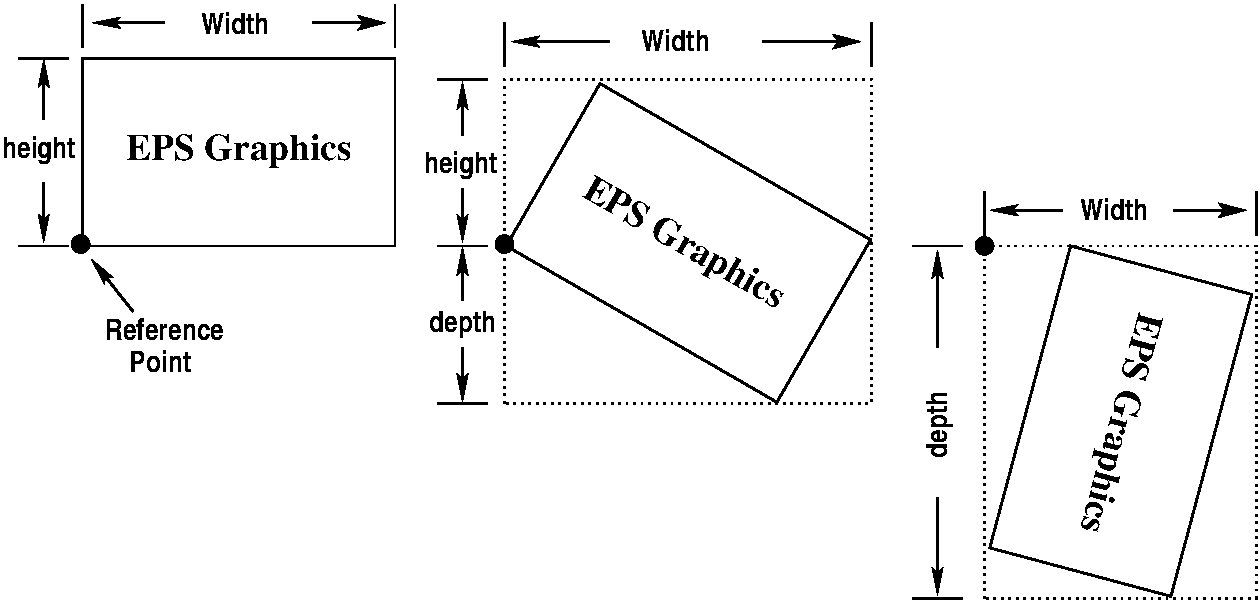
\includegraphics[width=.9\linewidth]{rotat-box}
	\caption{\LaTeX{}~盒子的旋转示例}\label{fig:rotate-box}
\end{figure}


============================
\section{Encapsulated PostScript}\label{sec:eps}

\PS~语言能够用来描述图形和文本。它既可在传统的~\PS{}(PS)~文件中来描述多页的
文档,也用于~Encapsulated \PS{}(EPS)~文件中来描述插入文档的图形。
PS~和~EPS~主要的区别在于:

\begin{minipage}{.9\linewidth}
	\noindent
	\begin{itemize}
		\item EPS~文件仅仅使用部分特定的~\PS~操作符。
		\item EPS~文件必须含有一个~BoundingBox~行来确定~EPS~图形的大小。
	\end{itemize}
\end{minipage}

\subsection[禁止使用的~\PS{}~操作符]{禁止使用的~~\PS{}~~操作符}\label{ssec:forbidps}

由于~EPS~图形需要和其它对象一起共享页面,所以~EPS~文件中不能使用像
选择页面大小~(\texttt{a4}~或~\texttt{letter})~和清除整个页
面~(\texttt{erasepage})~等命令。下面是一些不能在~EPS~文件中使用的~\PS{}~操作符:

\vspace{0.6cm}

\texttt{
	\begin{tabular}{llll}
		a3   &  a4 &  a5 &   banddevice  \\
		clear & cleardictstack & copypage &  erasepage \\
		exitserver & framedevice & grestoreall & initclip \\
		initgraphics & initmatrix & letter & legal \\
		note & prenderbands & quit & renderbands \\
		setdevice & setglobal & setpagedevice & setpageparams \\
		setsccbatch & setshared & startjob & stop \\
\end{tabular}}

\clearpage

尽管下列~\PS{}~操作符可以在~EPS~文件中使用,但是不适当的使用它们极易
导致错误。

\texttt{
	\begin{tabular}{llll}
		nulldevice & setcolortransfer & setgstate & sethalftone \\
		setmatrix & setscreen & settransfer & undefinedfont \\
\end{tabular}}

上面的一些操作符可能会使~DVI~到~PS~的转换失败,另一些则可能导致像
图形位置错误或图形消失等奇怪的问题。因为这些操作符绝大部分不会影响
到~\PS{}~的堆栈,所以,在大多数情况下,简单的将这些招致问题的操作符
删除就可解决问题。其它的情形则需要更为复杂的~\PS{}~的知识。

\subsection[The EPS BoundingBox]{The EPS BoundingBox}\label{ssec:bbox}
\index{EPS BoundingBox}

习惯上,\PS{}~文件的第一行是标明该文件的类型,接下来的几行是
被称为~\wi{header}~或~preamble~的注释行(~\PS{}~的注释符也是~\%)。
这些注释中的一行就定义了~BoundingBox~。BoundingBox~这行有四个整数值,
分别代表:

\begin{minipage}{.9\linewidth}
	\noindent
	\addtolength{\itemsep}{-5pt}
	\begin{enumerate}
		\item BoundingBox~的左下角的~$x$~坐标。
		\item BoundingBox~的左下角的~$y$~坐标。
		\item BoundingBox~的右上角的~$x$~坐标。
		\item BoundingBox~的右上角的~$y$~坐标。
	\end{enumerate}
	\addtolength{\itemsep}{5pt}
\end{minipage}

\vspace{1cm}

\begin{Verbatim}[frame=single,rulecolor=\color{mygreen},%
label={\CJKfamily{hei} EPS~文件头示例}]
%!PS-Adobe-2.0 EPSF-2.0
%%Creator: gnuplot
%%DocumentFonts: Times-Roman
%%BoundingBox: 50 50 410 302
%%EndComments
\end{Verbatim}

上面的例子是一个由~\texttt{gnuplot}~生成的~EPS~文件的前五行。
这个~EPS~图形的左下角的坐标是~$(50,50)$,
右上角的坐标是~$(410,302)$。这里坐标的单位是~\PS{} point,
等于~$\nicefrac{1}{72}$~英寸。这样上面的这幅图的自然宽度为~$5$~英寸,
相应的自然高度为~$3.5$~英寸。需要注意的是~\PS{} point~要比
~\TeX{} point~(等于~$\nicefrac{1}{72.27}$~英寸)稍大,
在~\TeX{}~和~\LaTeX{}~中,\PS{} points~被称为~``big points''~或简称
~\texttt{bp},~\TeX{} point~被称为~``points''~或简称~\texttt{pt}。

\subsection[将~PS~转换为~EPS]{将~~PS~~转换为~~EPS}\label{ssec:pstoeps}

单页的~\PS{}~文件,如果没有包含不适当的命令的话,可用下述方法转为
~EPS~文件并加上~BoundingBox。{\CJKfamily{hei} 由于这些方法
	都不检查非法的~\PS{}~操作符,所以只有在被转换的~\PS{}~文件本身
	不含有那些被禁制使用的操作符的情况下,才能得到正确的~EPS~文件。}
\begin{enumerate}
	\item 最方便的是用~\GS{}~里带的~\texttt{ps2epsi}~(见
	第~\ref{chap:gs}~章)。它可以读入~\PS{}~文件并
	计算~BoundingBox~的参数,然后生成一个含有~\PS{}~图形
	的~EPS~文件。
	
	最终得到的~EPS~文件是~EPSI~格式,即它在文件的开始部分
	带有一个底分辨率的预览位图。因为这个预览位图是~ASCII~编码
	的,所以不会造成像第~\ref{sec:linebuffer}~节的~\texttt{bufsize}~
	错误。不过,它却使得文件变大。\index{bufsize@\texttt{buffersize}}
	\item 另一种方法是计算~BoundingBox~的参数,然后把它加到~\PS{}~文件中
	或作为插图命令的参数(比如用~\cmd{includegraphics}~的
	~\texttt{bb}~方式)。计算~BoundingBox~的方法有以下几种:
	\begin{enumerate}
		\item 用~Ghostview~或~GSview~将~\PS~图形打开,当鼠标在
		图形上移动时就会显示相应的坐标(以页面的左下角为参照点)。
		记下图形的左下角和右上角的坐标就可确定它的~BoundingBox。
		\item 将~\PS~图形打印一份,测量它的左下角和右上角到页面的左下角                       的水平和垂直距离(以英寸为单位),然后乘以~$72$~就可得到
		它的~BoundingBox。
		\item 使用~\texttt{bbfig}。\texttt{bbfig}~是一个脚本文件,
		它在~\PS{}~图形文件前面加入一些~\PS{}~命令并送往
		~\PS{}~打印机。这时加入的命令会计算~BoundingBox,
		然后将结果打印在~\PS{}~图形上面。
	\end{enumerate}
\end{enumerate}

\clearpage

\subsection[修正非标准的~EPS]{修正非标准的~~EPS}\label{ssec:fixeps}

一些应用程序生成的非标准的~EPS~文件,另一些应用程序则根据它们自己
的喜好来加入一些~\PS~的``增强''功能,还有一些应用程序生成非常糟糕的
~\PS~代码。而由此得到的~EPS~文件是不能在~\LaTeX{}~中使用的。所幸
的是有许多有用的工具来修正这些非标准的~EPS~文件。

\begin{description}
	\item [Mathematica] 由~Mathematica 2.x~生成的~EPS~文件是用~Mathematica~
	的扩展~\PS~写成的。在非~Mathematica~程序使用这些~EPS~文件时,
	必须要把那些非标准的扩展代码去掉才行。~DOS~版本的~Mathematica 2.x~
	带有一个名为~\texttt{printps.exe}~或~\texttt{rasterps}~的工具
	可以将那些非标准代码去掉。对于~Unix~版本的~Mathematica 2.x~,
	这个任务可由~\texttt{psfix}~来完成。参考你的~Mathematica~文档
	或与~Wolfram Research~联系来获取进一步的信息。
	\item [FrameMaker] 由~FrameMaker~生成的~\PS~文件没有遵循~Adobe~的
	与纸张无关的声明。~Framemaker 4~和~5~生成的~\PS~文件可分别用
	下列脚本来修正:\\
	\href{ftp://ftp.irisa.fr/pub/FrameMaker/Filters/fixfm4-1.3.tar.gz}%
	{\texttt{ftp://ftp.irisa.fr/pub/FrameMaker/Filters/fixfm4-1.3.tar.gz}}\\
	\href{ftp://ftp.irisa.fr/pub/FrameMaker/Filters/fixfm5-2.0.tar.gz}%
	{\texttt{ftp://ftp.irisa.fr/pub/FrameMaker/Filters/fixfm5-2.0.tar.gz}}
	
	修正~Framemaker 3~和~4~生成的~\PS~文件的脚本~\texttt{fixfm3ps.sh}~和
	~\texttt{fixfm4ps.sh}~可从下面的地点得到:
	
	\href{ftp://ftp.frame.com/pub/techsup/framers/platform.ind/filters/}{\texttt{ftp://ftp.frame.com/pub/techsup/framers/platform.ind/filters/}}
	
\end{description}

\section[怎样在\LaTeX{}中使用~EPS~图]{怎样在~~\LaTeX{}~~中使用~~EPS~~图}\label{sec:useeps}

EPS~文件能被~\LaTeX{}~和~DVI~到~PS~的转换程序使用。

\begin{enumerate}
	\item \LaTeX{}~通过读取~EPS~文件中的~BoundingBox~行来决定为~EPS~图形
	保留多大的空间。
	\item DVI~到~PS~的转换程序读取~EPS~文件并把它插入到生成的~PS~文件中。
\end{enumerate}

需要说明的几种情形:

\begin{itemize}
	\item 如果在图形插入命令中给定了~BoundingBox~的值,~\LaTeX{}~将不会从
	~EPS~文件读取它的~BoundingBox~行。
	\item 由于~\TeX{}~不能读取非~ASCII~文件,也不能生成其它的程序,所以
	~\LaTeX{}~不能从压缩的~EPS~文件或其它非~EPS~文件中得到~BoundingBox~
	的信息。在这种情况下,可以在图形插入命令中给定~BoundingBox~的值
	或将~BoundingBox~的值放到一个文本文件中(见第~\ref{chap:noneps}~章)
	\item ~EPS~图形并没有被加到~DVI~文件中,它是在从~DVI~到~PS~转换时才被
	加到生成的~PS~文件中的。因此,所有用到的~EPS~文件必须和~DVI~文件
	在一起。
	\item 大多数旧版本的~DVI~浏览器不支持显示~EPS~图形。这时,~DVI~浏览器
	一般会将~EPS~图形的~BoundingBoX~用一方框显示出来,以方便使用者
	对图形进行定位。目前版本的一些~TeX~软件如~Mik\TeX{}~、~fp\TeX{}~和
	~te\TeX{}~等所带~DVI~浏览器(\texttt{Yap, Windvi, Xdvi})可以借助
	于~\texttt{ghostscript}~来显示~EPS~图形。
\end{itemize}

\subsection[行缓冲区溢出]{行缓冲区溢出}\label{ssec:linebuffer}

\LaTeX{}~在读取~ASCII~文件时是每次从中读取一行,然后把它放到自己
的行缓冲区里。~\LaTeX{}~的行缓冲区大约有~3000~字节。如果~EPS~文件中
有一行的长度超过了行缓冲区的长度,就会产生如下的错误讯息:

\begin{Verbatim}[xleftmargin=22pt]
Unable to read an entire line--bufsize=3000.
Please ask a wizard to enlarge me.
\end{Verbatim}

因为~EPS~很少有一行长度超过~3000~字节的情形,所以产生行缓冲区溢出
的原因可能有两种:

\begin{enumerate}
	\item {\CJKfamily{hei} EPS~文件中有一个长的二进制的预览图}
	
	有些应用程序生成的~EPS~文件在开始部分放置了一个二进制的预览图,
	这样就可使得像~DVI~浏览器等一些不能解释~\PS~的软件也可来显示
	~EPS~图形。目前有少数与~\TeX{}~有关的软件使用这种方法。
	
	如果这个二进制的预览图比行缓冲区小,~\cmd{includegraphics}~将会
	略过它(像~\cmd{psfig}~等过时的命令则不会这样)。但是,如果这个
	二进制的预览图比行缓冲区大的话,就会发生行缓冲区溢出的错误。
	有两种解决办法:
	
	\begin{enumerate}
		\item 如果不需要预览图,可以用文本编辑器将它删掉或在生成~EPS~
		图形时就选择不要预览图。
		\item 因为~\LaTeX{}~读取~EPS~文件的唯一目的就是取得~BoundingBox~
		的大小,故可在插图命令中给出~BoundingBox~
		的值(如在~\cmd{includegraphics}~中使用~\texttt{bb}~选项)
		从而使得~\LaTeX{}~不再读取~EPS~文件。
	\end{enumerate}
	
	\item {\CJKfamily{hei} ~EPS~文件中的分行符在不适当的传输中被损坏}
	
	(这里所谈到的问题不会在一些最新版本的~\TeX{}~软件中出现,因为这
	些软件中的~\TeX{}~都会正确的识别所有的分行符。)
	
	不同的操作系统平台使用不同分行符。~Unix~使用~\verb+^J+,
	~Macintosh~使用~\verb+^M+,而~DOS/Windows~则使用~\verb+^M^J+。
	比如一个~EPS~文件从~Macintosh~机上用二进制方式传输到~Unix~机上,
	那么~Unix~机上的~\TeX{}~会因找不到分行符~~\verb+^J+~而把整个文件
	作为一行,导致行缓冲区溢出的错误。
	
	如果~EPS~文件中不含有二进制的部分(如预览图和嵌入的图形),以文本
	方式传输就可以解决这一问题。否则,由于文件必须用二进制方式传输,
	分行符的问题不可避免,这时就需要用一些工具来转换不同的格式或在
	在插图命令中给出~BoundingBox~的值来解决。
\end{enumerate}

\section[下载和安装\GS]{下载和安装~~\GS}\label{sec:gs}

\GS~是一个~\PS~语言解释器,它可以运行在大多数操作系统平台上并由~Aladdin
Enterprises~自由\realfootnote{Although Aladdin Ghostscript is distributed for
	free, it is not in the public domain. It is copyrighted and comes with
	certain limitations such as no commercial distribution. When versions of
	Aladdin Ghostscript become approximately one year old, Aladdin releases
	them as ``GNU Ghostscript'' whose use is governed by the less-restrictive
	GNU Public License.}发放。通过~\GS~可以在屏幕上显示~\PS~和~EPS~文件,也可
用非~\PS~打印机来打印。~Aladdin \GS~可从
~\href{ftp://ftp.ctan.tug/tex-archive/supported/ghostscript/aladdin/}%
{\texttt{CTAN/supported/ghostscript/aladdin/}}~取得。也可直接访问~\GS~的
主页:
\begin{quote}
	\href{http://www.cs.wisc.edu/~ghost/index.html}{\texttt{http://www.cs.wisc.edu/~ghost/index.html}}
\end{quote}
这一~Web~网址提供了比~CTAN FTP~站点更多更好的相关信息。
这些站点都提供~Windows/DOS/OS{\small /}2~和~Macintosh~的可执行文件,
~Unix/VMS~下的源代码。同时,还能下载~\GS~的图形用户界面(~Windows/OS/2~下
的~GSview~和~Unix/VMS~下的~Ghostview),这将使你更容易的观看和打印~\PS~文件。

Aladdin \GS~目前的正式版本为~6.01,~GNU \GS~的正式版本为~5.50。
对于~Window/DOS/OS{\small /}2~和~Macintosh~的用户来说,直接下载
它的已编译好的压缩包,安装使用就行了。而对于~Unix/VMS~的用户,通常
需要自己编译。编译时,首先将~\texttt{ghostscrip-x.xx.tar.gz}~和
其它所需的软件包解压缩:
\begin{Verbatim}[xleftmargin=1cm]
gzip -dc ghostscrip-x.xx.tar.gz | tar -vxf -
cd gsx.xx
gzip -dc ghostscrip-x.xxjpeg.tar.gz | tar -vxf -
gzip -dc ghostscrip-x.xxlibpng.tar.gz |tar -vxf -
gzip -dc ghostscrip-x.xxzlib.tar.gz | tar -vxf -
\end{Verbatim}
解压后可参考~GS~所带的帮助文件~make.txt~来按照你的要求编辑适当的~.mak~
文件,然后进行编译(假设使用~\texttt{gcc}~编译)和安装:
\begin{Verbatim}[xleftmargin=1cm]
ln -s src/gcc.mak ./Makefile
make
make install
\end{Verbatim}

\GS~中还带有一些有用的工具,如~\texttt{ps2pdf}~等,可利用~GS~来
转换图形,打印、预览~\PS~文件。详细的使用说明可参考~GS~所带的
使用说明文件。

\section{图像格式转换工具}\label{sec:convertor}

下面列出的一些免费软件和共享软件可以用来将非~EPS~格式的图形
转换为~EPS~图形。其中一部分提供命令行方式的软件,在用~\texttt{dvips}~
将~DVI~转为~PS~的过程中能同时自动转换图形的格式。具体见第~\ref{sec:noneps}~节。

\begin{itemize}
	\item \texttt{ImageMagick}~是一个很好的图形转换工具,可从
	~\href{ftp://ftp.wizards.dupont.com}{\texttt{ftp.wizards.dupont.com}}~或
	其它站点自由下载。参见:
	
	\href{http://www.wizards.dupont.com/cristy/ImageMagick.html}%
	{\texttt{http://www.wizards.dupont.com/cristy/ImageMagick.html}}
	
	除~Unix~和~Linux~外,它也可运行在~Windows NT, Macintosh~和~VMS~下。
	
	\item \texttt{xv}~是一个~\$25~的共享软件,运行在~X-Windows~环境下,可
	用来观看和转换图形。~\texttt{xv}~没有命令行方式,因此无法利用她来
	实现图形格式的即时转换功能。有关~\texttt{xv}~的信息可参见:
	
	\href{http://www.sun.com/sunsoft/catlink/xv/note.html}%
	{\texttt{http://www.sun.com/sunsoft/catlink/xv/note.html}}
	
	\texttt{xv}~的在线手册:
	
	\href{http://is.rice.edu/~shel/xv-3.10a/}{\texttt{http://is.rice.edu/~shel/xv-3.10a/}}
	
	\item \texttt{DISPLAY}~是~DOS~下的免费软件,能够转换多种图像格式。
	可从下面的地点下载~\texttt{disp189a.zip}~和~\texttt{disp189b.zip}~
	(新的版本可能不是~\texttt{189}~。)
	
	\href{http://www.simtel.net/simtel.net/msdos/graphics-pre.html}%
	{\texttt{http://www.simtel.net/simtel.net/msdos/graphics-pre.html}} \\
	\href{http://www.simtel.net/simtel.net/msdos/graphics-pre.html}%
	{\texttt{http://www.simtel.net/simtel.net/msdos/graphics-pre.html}}
	
	\item \texttt{WMF2EPS}~运行在~Windows9.x/NT~下的将~WMF~格式的图像转为~EPS~
	格式的免费软件。参考以下文件来取得这一软件。
	
	\href{ftp://ftp.tug.org/tex-archive/support/wmf2eps/readme.txt}%
	{\texttt{CTAN/support/wmf2eps/readme.txt}}
	
	它需要你的系统中装有~Adobe~兼容的打印机驱动。
	
	\item \texttt{KVEC}~是一个~\$25~的共享软件,能够将位图格式的图形(BMP, GIF,
	TIFF)等转为~\PS~或其它矢量图形。~\texttt{KVEC}~可运行在~Windows, OS/2,
	NEXT~和~Unix~下。
	
	\href{http://ourworld.compuserve.com/homepages/kkuhl/}%
	{\texttt{http://ourworld.compuserve.com/homepages/kkuhl/}}
	
	\item \texttt{NetPBM}~是旧有的~\texttt{PBMPLUS}~工具包的保留和扩充。
	目前它可运行在~Windows, Unix, VMS, DOS~等多种平台下。
	
	\href{http://wuarchive.wustl.edu/graphics/graphics/packages/NetPBM/}%
	{\texttt{http://wuarchive.wustl.edu/graphics/graphics/packages/NetPBM/}}
	
	\item \texttt{ImageCommander}~(共享软件,~\$19)是~Windows3.1/95/NT~下的
	图形转换软件,可将~GIF, JPEG, PICT, WMF~等多种图形转换为~EPS~和其它
	格式的图形。更详细的信息可见:
	
	\href{http://www.jasc.com/}{\texttt{http://www.jasc.com/}}
	
	JASC~的~Paint Shop Pro 绘图软件(共享软件,~\$69)具有同样的图形转换
	功能。
\end{itemize}

\subsection[Level 2 EPS~封装]{Level 2 EPS~封装}\label{ssec:epswrapper}

与传统的~\PS~不同的是,~Level 2 \PS~支持压缩的二进制图形。
这使得它能够制作出比传统的~EPS~更小、质量更好的图形。
如果你有一台~Level 2 \PS~打印机,那么你最好是用下面的
这些封装程序来替代上节中的那些转换软件。不过由于这样得到的~\PS~文件
只能在~Level 2 \PS~打印机上打印,会降低文件的通用性。

\begin{itemize}
	\item \texttt{jpeg2ps}~是一个用~C~语言程序,可将~JPEG~图形转换为~Level 2 \PS~
	图形。\texttt{jpeg2ps}~可在~Unix, DOS~和其它操作系统下使用。
	
	\href{http://www.muc.de/~tm/free/free.html}{\texttt{http://www.muc.de/~tm/free/free.html}}
	
	\item TIFF~图形可用~\texttt{tiff2ps}~转换为~LZW--编码的~Level 2 \PS~。
	\texttt{tiff2ps}~的源代码在:
	
	\href{ftp://ftp.sgi.com/graphics/tiff/tiff-v3.4-tar.gz}%
	{\texttt{ftp://ftp.sgi.com/graphics/tiff/tiff-v3.4-tar.gz}}
	
	\texttt{tiff2ps}~能在~Unix, DOS, Mac~和~VMS~下编译成功。尽管
	~LZW \PS~文件较小,但是它需要~~Level 2 \PS~打印机。
\end{itemize}

\subsection[编辑\PS]{编辑~~\PS}\label{ssec:editps}

虽然可直接编辑~EPS~文件中的~\PS~命令来改变图形,但这对一些不熟悉
~\PS~语言的人来说还是很困难的。所幸的是,借助于下面的一些工具软件,
可以很容易的编辑~EPS~图形。

\begin{itemize}
	\item \texttt{pstoedit} 是~Unix, Windows, DOS~和~OS/2~下的免费软件,
	借助于~\GS,它能购将~\PS~或~PDF~图形转为其它矢量格式(比如~
	\texttt{xfig}~的~\texttt{.fig}~格式)。~\texttt{pstoedit}~的
	C$++$~源码可从下述站点取得。
	
	\href{ftp://ftp.x.org/contrib/applications/pstoedit/pstoedit.html}%
	{\texttt{ftp://ftp.x.org/contrib/applications/pstoedit/pstoedit.html}}\\
	\href{http://www.geocities.com/SiliconValley/Network/1958/pstoedit/}%
	{\texttt{http://www.geocities.com/SiliconValley/Network/1958/pstoedit/}}
	
	\item \texttt{Mayura Draw}~(以前称为~\texttt{PageDraw})是~Windows3.1/9.x/NT~
	下的绘图软件。当与~\GS~一起使用时,它可以编辑~\PS~文件。见:
	
	\href{http://www.wix.com/PageDraw}{\texttt{http://www.wix.com/PageDraw}}
	
	旧版本的~\texttt{Mayura Draw}~是免费软件,最近的版本则为~\$15~的共享
	软件。~\texttt{Mayura Draw}~需要~Adobe Type Manager (ATM)~来在图形上
	放置文本。虽然~ATM~现在是商业软件,但是~Adobe~在~Acrobat Reader 2.0~中
	提供了一个免费版本。
	
	\href{ftp://ftp.winsite.com/pub/pc/win3/util/acroread.zip}%
	{\texttt{ftp://ftp.winsite.com/pub/pc/win3/util/acroread.zip}}
	
	\item \texttt{xfig}~是~Unix/Xwindows~下功能强大的免费绘图软件,能够
	引入~EPS~图形并加上标记。不过目前还不能改变原始的~EPS~图形。
	访问~\texttt{xfig}~的主页获取更进一步的信息。
	
	\href{http://www.xfig.org/}{\texttt{http://www.xfig.org/}}
	
\end{itemize}

\clearpage
\vbox to .5\textheight{\mbox{}}
\clearpage

\endinput
